% A simple LaTeX template for lab reports in TDT4258 Energy Efficient Computer Design
% by Yaman Umuroglu (yamanu@idi.ntnu.no)
% Feel free to customize the style as you see fit, but the chapters/sections mentioned in the
% template should be included with the appropriate content.

\documentclass[abstract=on]{scrreprt}
\usepackage[utf8]{inputenc}


\usepackage{natbib}
\usepackage{graphicx}
\usepackage{listings}
\sloppy

\usepackage[parfill]{parskip} %Skip-line-paragrafer i koden blir skip-line-paragrafer i dokumentet


% Edit the meta.tex file to change title, group number and author names
% Fill in the report title, group number and student names here
\newcommand{\mytitle}{Exercise - 3}
\newcommand{\mygroupnumber}{4}
\newcommand{\myauthor}{Erlend Hestnes\\Christoffer Ramstad-Evensen\\Jon Zwaig Kolstad}

\title{\mytitle}
\author{\myauthor}
\date{\today}



\begin{document}
% The title page, edit if you want to customize it
\begin{titlepage}

\includegraphics[height=1.5cm]{images/ntnu_logo.pdf}\\[1cm]   
\begin{center}

 
% Upper part of the page
~\\[1.5cm]

\textsc{\Large TDT4258 Energy Efficient Computer Design\\Laboratory Report}\\[0.5cm]

% Set the title of the Document between two horizontal lines
\hrule ~\\[0.2cm]
{\huge \bfseries \mytitle}\\[0.4cm]		% print the title of the document
\hrule ~\\[1.5cm]

% Additional Information about the document
\begin{minipage}{0.4\textwidth}
    \centering
	\large
		\emph{Group \mygroupnumber:}\\~\\
		\myauthor
\end{minipage}

\vfill

% Bottom of the page
{\large \today}

\end{center}
\end{titlepage}


% Main matter - edit corresponding file under content/ to change
\begin{abstract}

This report explores the possibility of using a Linux distribution for a relatively small embedded computer system. A simple game of Pong has been created as demonstration for this project. An interrupt based Linux device driver has been implemented for the game pad that controls the game. The report further investigates the energy aspects of using Linux on an embedded platform. The results clearly show that using such a complex system takes away some flexibility in regards of tailoring an applications to meet a specific need. An average current consumption of 12 mA was achieved. 

\end{abstract}
\tableofcontents
\chapter{Introduction}

The embedded industry is currently undergoing a fundamental change. Nearly all of the big semiconductor corporations are moving away from the traditional 8-bit cores (8051, AVR, MSP430 etc.), and over to more advanced 32-bit ARM based cores. The marked is in demand of connectivity and processing power, areas where the 8-bit cores struggles. One downside of this migration, is that the complexity of designing embedded software increases. The 8-bit cores were so simple to program that an operating system was unnecessary in most cases, while high level application programming interfaces (API)'s are almost essential for a 32-bit architecture. As a result of this, we are beginning to see more and more embedded systems running operating systems. This is great news for the designer, since it makes it much easier to develop complex applications. However, the introduction of high level API's has it's downsides. Designers have less control over whats going on under all the software layers, giving them less flexibility to tailor their applications to suit their specific needs, which in essence is what embedded systems are all about.

The report explores the concept of running a Linux distribution on a relatively small embedded system. The report elaborates on the pros and cons with using such a system to design a simple game of Pong. As well as some aspects in regards to power consumption. The results show the developer can significantly reduce the overall development time 



\chapter{Background and Theory}

The achieved implementation consist of many different components including hardware (HW), advanced energy monitoring tools, Linux build systems and other software such as drivers. This section will elaborate on the specifics of the HW platform as well as the Linux build system and, the uClinux distribution and drivers necessary for controlling a Pong game with an external gamepad.

\section{EFM32GG}
The EFM32GG by Silicon Labs is a 32-bit MCU, and the best of its class in their range, based on its specifications \cite{SLABSMCUS}. It packs an ARM Cortex-M3 central processing unit (CPU), various peripherals, loads of general purpose IO (GPIO), 64–256 kB flash storage and 128 kB of RAM. One of the main advantages of using the EFM32GG, are the Energy Modes (EM) which are effective tools to control power consumption. \\

\section{DK3750}
The DK3750 development kit is a modular motherboard with detachable modules for a CPU board and different prototyping boards. The motherboard features buttons, LEDs, extra flash storage, extra RAM, an SD-card slot, Ethernet- and RS232-port, analog input and output jacks, a USB host connector, plenty of GPIO, and a 3.5" TFT-LCD display with a joystick.\cite{DK3750RM}

\section{Advanced Energy Monitoring}
Advanced Energy Monitoring (AEM) is a feature realized by the DK3750 board controller and the Silicon Labs software, Energy Profiler. It measures the MCU's current consumption in real-time. An option to show energy on the TFT-LCD display comes shipped with the kit. To enter this mode, just turn on the kit and push the appropriate button beneath the screen. 

\section{ARM Cortex-M3}
The ARM Cortex-M3 features a 3-stage pipeline-, Modified Harvard-, and RISC-processor architecture \cite{CORTEXM3RM}. A 3-stage pipeline is equivalent to the processor operating simultaneously on three instructions: One being fetched, another being decoded and the last being executed. Harvard architecture means having separate buses for instructions and data memory, enabling accesses to each space to happen concurrently. This greatly benefits performance. Reduced instruction set computing (RISC) architecture involves a process with a minimum number of instructions that can further make up other functions. \texttt{Load/store} are the only explicit instructions that references memory, all other instructions are handled inside internal registers. This, together with simple hardware (compared to CISC), is a core advantage of the RISC-architecture. When the three properties mentioned here are combined, they enable more work to be done in a single clock cycle, which further contribute to faster performance and a reduced demand for power. 

\section{Ptxdist Build System}

The Linux distribution is built with a build system called ptxdist. This system compiles and builds the kernel, the modules and other software programs. The results of the build is binary files that can be flashed to the development board. To use ptxdist it must be specified a configuration that defines the applications which are to be built for the HW platform. The setup is completed by specify a HW platform and the toolchain \cite{ptxsetup}. For more information on the workflow of ptxdist please refer to "Overview of ptxdist and build system - Lab Exercises in TDT4258 Energy Efficient Computer Systems" \cite{COMPENDIUM}.

\section{uCLinux}

uCLinux is a Linux distribution aimed specifically at small embedded computer systems. The kernel itself can use as little as 330K of flash, although this number usually exceeds a few megabytes when additional peripheral drivers are included . The distribution also needs a few megabytes of RAM to function properly. The EFM32GG is only equipped with 1MB of flash and 128kB of RAM, which is a little low to run uCLinux. However, the DK3750 has 16MB flash and 4MB of RAM connected to the EFM32GG through the external bus interface (EBI) \cite{DK3750RM}. By using this extra memory, the EFM32GG is able to run uCLinux with no problems.  

The main difference between a fully fledged Linux distribution and uCLinux is the lack of an memory managment unit (MMU). This makes the use of virtual memory (VM) impossible. When using VM, all of the processes run in the same virtual address space. This enables the possibility of using contiguous virtual memory, scattered physical pages and adding memory to an already running process.

With no VM, all memory allocated to a process must be contiguous. This might cause fragmentation problems, especially for configurations that spawns many processes dynamically. Luckily, embedded systems often tend to have static process, which mitigates the fragmentation problem of not having an MMU.   

\section{Framebuffer}

The LCD display on the DK3750 was used for this project. The LCD display has a resolution of 320x240 pixels, and a color depth of 16-bit. The display can either be driven by the on-board SSD2119 display controller, or by using direct drive mode from the EFM32GG. In both cases, data is sent as 16-bit RGB format. The data is organized as shown in Figure \ref{fig:display_format}. 

\begin{figure}[h]
\centering
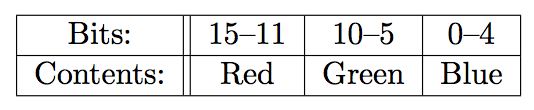
\includegraphics[width=0.6\textwidth]{images/display_format.png}
\caption{Organisation of each pixel in the framebuffer. \cite{COMPENDIUM}}
\label{fig:display_format}
\end{figure}

A pre-made Linux device driver was used to communicate with the display. The device driver utilizes a frame buffer, as depicted in Figure \ref{fig:framebuffer}. A simple API was implemented in ANSI C for this driver. The API features functions for drawing simple geometric shapes and text on the display.  

\begin{figure}[h]
\centering
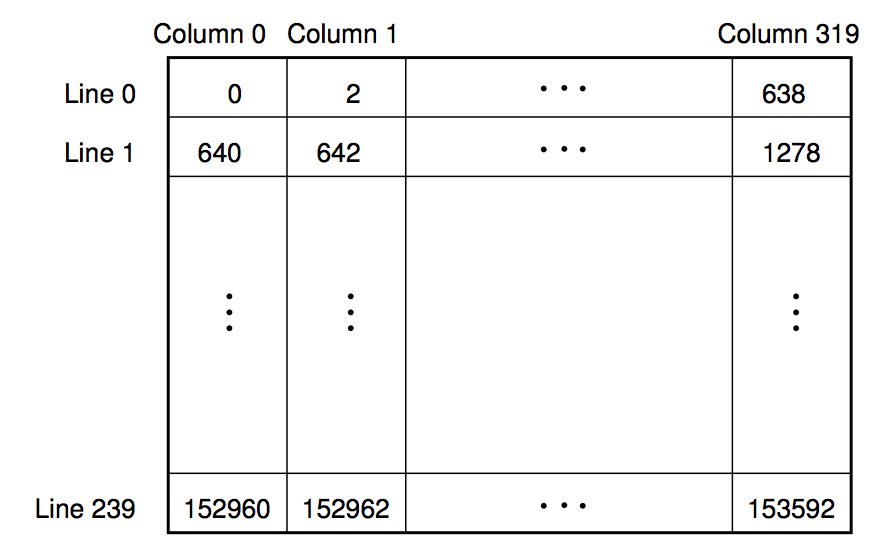
\includegraphics[width=0.6\textwidth]{images/framebuffer.png}
\caption{Organisation of ramebuffer. Each square corresponds to one pixel and the address of this pixel. \cite{COMPENDIUM}}
\label{fig:framebuffer}
\end{figure}


%Loadable kernel module
%Interface between kernel and module
%Ptxdist

\section{Device Drivers}

This section is an introduction to the fundamentals of a device driver, especially Linux device drivers, and how a char device driver is implemented in a Linux environment. It will also elaborate on how interrupts can asynchronously notify processes through a device driver.

\subsection{What is a Device Driver?}

A device driver \cite{devicedriver} is a software program which delivers an interface between operating systems (OS) and HW devices connected to it. This is convenient when programs run by the OS should access the HW and don't have to bother with complex HW functions and memory allocation. From the OS's point of view there should be a ``black box'' between its interface and the HW.

\subsection{Linux Device Drivers}

In the Linux environment device drivers are implemented as modules which is a piece of code added to the kernel at runtime \cite{module}. This module defines the driver methods, registers the driver, allocates an appropriate memory region for the device and handles the HW functions \cite{ch3}. Driver methods are the functions available for the invoker of the driver. When registering a driver, different entries for the driver are made in the file system, and especially the driver could be made available in User Space in the \emph{/dev} directory.

Different device drivers are often put in three classes \cite{classes}: \emph{Char device, Block device and Network interface}. This report will focus on the Char device as this was implemented in the final solution. 

\subsection{Char Device Drivers}

%A Char device is a device that needs to be accessed in a byte stream oriented way \cite{classes}. 

The setup of a char device driver consists of a routine to be executed when loaded and unloaded from the kernel. This is achieved through an \emph{init} and \emph{exit} function \cite{initexit} inside the driver. The \emph{init} function includes most of the setup for communicating with the device and creating the device in the kernel file system. The \emph{exit} function ensures that the driver is completely removed from the kernel and all structures and memory regions are released. 

One of the most important structures inside the driver is the file operation structure \cite{fops}. This structure holds the methods of the driver such as \emph{open, close, release, write} and \emph{fasync}. The methods \emph{open, close, release} and \emph{write} handles the system calls \emph{open, close, read} and \emph{write}. This lets applications in user space access the driver through shell command as \emph{echo} or \emph{cat}, in example. The \emph{fasync} \cite{fasync} method enables asynchronous notification between the driver and the invoking process. 

Since the creation of the device happens in the \emph{init} function there are a few necessary steps which must be included in this function. First the device is registered to the kernel and assigned a major number so that the driver can be identified to a device \cite{major}. Calling the function \texttt{alloc\_chrdev\_region} \cite{region} registers the device and dynamically allocates a major number for use through the creation of the device. In order to create the device a class structure has to be initialized with the function \texttt{class\_create} \cite{class}. Now the device can be created by calling \texttt{device\_create} \cite{devcreate} and passing a pointer from the class structure as an input parameter. The device is then initialized and added to the kernel with the \texttt{cdev\_init} \cite{cinit} and the \texttt{cdev\_add} \cite{cadd} functions. Now the device is created in the kernel file system and the driver instance is found in the \emph{/dev/} directory. Additional setup, such as requesting memory for the device, is also to be put in the \emph{init} function.

When the driver is unloaded from the kernel the call to the \emph{exit} function must ensure the release of all the resources setup for the device. The \emph{exit} function should therefor delete the device and the class structure with the functions \texttt{device\_destroy} \cite{devdestroy} and \texttt{class\_destroy} \cite{classdestroy}. Before unregistering the char device with function \texttt{unregister\_chrdev} \cite{unregister} the cdev structure is deleted with the function \texttt{cdev\_del} \cite{cdel}.

For the driver to support interrupts through asynchronous notification an interrupt handling function and a function for the method \emph{fasync} is needed. All the necessary memory allocation and setup of interrupts are done in the \emph{init} function, but the signaling procedure are put in the interrupt handler. A call to the function \texttt{kill\_fasync} \cite{fasync} will signal the interested process of the occurrence of the interrupt. The \texttt{fasync\_helper} \cite{fasync} function is put in the \emph{fasync} method to register interested processes for asynchronous notification. To invoke this method the user space program must implement the code:

\begin{lstlisting}
    int oflags;
    descr = open("/dev/some-driver", O_RDONLY);
    signal(SIGIO, &interrupt_handler);
    fcntl(descr, F_SETOWN, getpid());
    oflags = fcntl(descr, F_GETFL);
    fcntl(descr, F_SETFL, oflags | FASYNC);
\end{lstlisting}

It is possible to copy memory of the device to user space by calling the function \texttt{copy\_to\_user} \cite{cpyusr}. This is often called when the \emph{read} method is called. 

%A Char device driver often implements functions for the four system calls \emph{open, close, read and write} which are used for communicating with the device. The driver also functions as a link between Kernel Space and User Space. The driver must implement a way to grant the request of Kernel Space data if it is intended by the driver to provide this for the User programs. 

%\subsection{Advanced Char Device Drivers}

%More advanced drivers provides more functionality as interrupt handling and asynchronous notification of other processes \cite{ch3}. 

\section{Pong}

Pong is a two-dimensional, table-tennis inspired arcade game, initially developed by Allan Alcorn, and released by Atari in 1972. It was a huge commercial success, and is considered to have had a great contribution towards the rise of the video game industry. 

The game 
\chapter{Methodology}

\section{Writing the Char Device Driver}

%This section elaborates on the necessary steps to create the device driver implemented in this design. 

The implemented char device driver support system calls such as \emph{open, close, read} and \emph{write} and enables asynchronous notification through the \emph{fasync} method. A file operations structure is declared to holds this functionality and refer them to the driver. An interrupt handler is setup to get input from the gamepad. 

The initialization setup is held in the \emph{init} function which includes the setup of the char device and the interrupts. The char device setup follows the necessary steps, as listed:
\begin{itemize}
\item Char device registration.
\item Class creation necessary for creating the device.
\item Creating the device and \emph{/dev/}-instance.
\item Initialize the char device and adding it to the kernel.
\end{itemize}
To enable the driver for interrupts the interrupt configuration registers are requested. The registers are set to enable interrupt on both falling and rising edge. 

The driver supports a routine for when the driver is unloaded from the kernel.
This is ensured by the \emph{exit} function which deallocates the requested memory region and deletes the device and all the structures used for device registration and class creation.

The driver supports user space functionality through the functions \emph{open, release, read} and \emph{write}.
The \emph{open} function requests interrupt handling for both EVEN and ODD pins and links the interrupts to the interrupt handler. Interrupt handling is disabled through the \emph{release} function.
The \emph{read} function reads the button register and sends a copy of the inverted values through an input variable. This enables user space application to read the button values into a buffer. The \emph{write} function is left empty as the driver does not support this functionality.
The \emph{open, release, read} and \emph{write} functions are linked to the file operations \emph{open, close, read} and \emph{write} respectively.

The \emph{fasync} method registers processes to the list of interested processes to be invoked by asynchronous notification. All interested processes are notified by the interrupt handler function. 

%\subsection{Old driver methodology}

%The \emph{init} function is were the main setup of the driver occurs. 
%First the char device is registered with a call to the function \texttt{int alloc\_chrdev\_region (dev\_t* dev, unsigned baseminor, unsigned count, const char* name)}. The char device is then registered with name and given a Major number. A call to \texttt{struct class* class\_create (struct module* owner, const char* name)} creates the class structure used to create the char device. Creating the char device and the \texttt{/dev/} instance is aquired by a call to \texttt{struct device* device\_create (struct class* class, struct device* parent, dev\_t devt, const char* fmt, ...)}. When the char device is created it is initialized and connected to the file operations with a call to \texttt{void cdev\_init (struct cdev* cdev, const struct file\_operations* fops)}. Complete the char device setup and adding the char device to the kernel with \texttt{int cdev\_add (struct cdev* p, dev\_t dev, unsigned count)}.

%To specify the functionality of the char device driver it is necessary to declare a structure for the file operations. The \emph{open, close, read and write} functions and the owner of the module are linked to this struct. 


%The \emph{exit} function is responsible of delete all structures and release the device driver from the memory.

%\subsection{Asynchronous Notification}

%The file operations struct used for the driver methods such as read, write, open and release, supports a method for asynchronous notification. This method can be used together with interrupts to signal a user space application. The user space application can then handle this interrupt accordingly. 

%To setup asynchronous notification it is necessary to call the \emph{fasync\_helper} function \cite{fasync} from within the fasync method of the file operations struct. This function is invoked when the FASYNC flag changes for an open file, in user space, and will add or remove entries from the list of interested processes \cite{fasync}. A call to the \emph{kill\_fasync} function will signal the processes or process group interested. Usual signal parameters for \emph{kill\_fasync} is SIGIO \cite{fasync}.

%Functions are included in $<linux/fs.h>$.

\section{Pong}

The actual game application is a simplified version of the famous arcade game, \textit{Pong}. Even though most implementations features a multi-player environment,  this game is designed only with a single-player mode. The goal of the game is simple: Prevent a constantly moving ball from leaving a room using a controllable bat. The room has three walls and an open edge. The bat is a static bar with the ability to move left and right along the open edge, located at the bottom. Upon hitting the ball with the bat, the ball's direction is changed relative to the distance from the middle of the bat, with a perfect hit sending the ball straight forward. The game is made more challenging by having the ball move faster the longer you prevent it from exiting the room. 
How can this game be designed to consume the least energy? There are several considerations that can be made, some are described in the following.

Pong is a dynamic game, meaning the ball will always be moving no matter what the user does. Because of this, the CPU can't be allowed to sleep when the user isn't doing anything because game data and output must be updated periodically. 

\section{Kernel ticker}

One problem with reducing the power consumption using Linux is the scheduler. The kernel maintains a so called "kernel ticker" which wakes up the kernel with a frequency of 100Hz \cite{tickless}. This is used to resume processes for which an timer related event has occurred. Waking the CPU at such a frequency is costly in terms of power consumption. Fortunately, the Linux kernel has the ability to enable a so called "tick-less kernel". In this scheme, the kernel calculates the time it needs to wake-up for the next event. By using this scheme, one reduces the number of timer interrupts drastically. Using the "tick-less kernel" option should contribute to lower the overall power consumption.

\section{Power Saving: Considerations}
%This section might not be necessary
uCLinux controls most of the EFM32GG subsystems, including the clock tree. Power saving techniques is therefore somewhat constrained to what the operating system actually supports. Fortunately, uCLinux is designed with energy efficiency in mind. 

\subsection{I/O Considerations}

Pong requires some kind of display for interaction and to show game objects such as ball and bat. Screens vary in resolution, pixel technology, color support, and brightness levels which further results in different energy demands for every screen. 

To print graphical objects or text on the screen, bits must be changed in the frame buffer. In order to see the change of bits on the screen, it must be refreshed. In order to achieve efficiency, refreshing should be done at a minimum. The game application is optimized to only refresh the display sections which has movement. This makes the refresh procedure very fast, which in term enables us to hibernate the CPU for several milliseconds between each screen refresh. This is also made possible by utilizing an interrupt based scheme for the game pad, so that CPU does not need to waste cycles to check for user input.  
\chapter{Results}
This section presents the results from the power consumption measurements. The results will be discussed and compared in terms of the different techniques used to make the game more power efficient.

The power consumption was examined with three different benchmarks. The first benchmark shows the power consumption without any sleep, and with the display refresh function set to refresh the entire display each time a change occurs. As seen from Figure \ref{fig:no_opt}, the average current consumption is 33mA.

\begin{figure}[h]
\centering
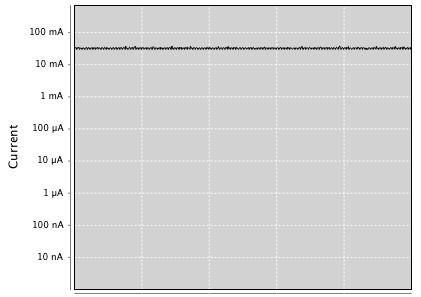
\includegraphics[width=0.5\textwidth]{images/welcome_no_opt.png}
\label{fig:no_opt}
\caption{Average current consumption of 33mA with game running with no optimizations.}
\end{figure}

The second benchmark shows the power consumption with sleep enabled in-between a display refresh. The display is still set to refresh the entire display when a change occurs. As seen from Figure \ref{fig:sleep}, the average current consumption is 30mA. This number underlines the cost of an entire display refresh.  

\begin{figure}[h]
\centering
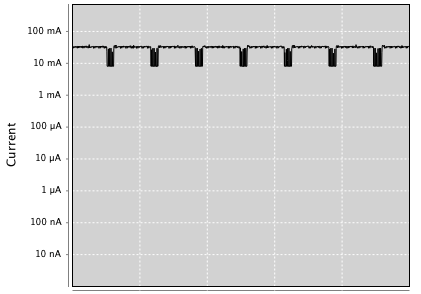
\includegraphics[width=0.5\textwidth]{images/welcome_sleep.png}
\label{fig:sleep}
\caption{Average current consumption of 30mA with game running with no optimizations but put to sleep for 50ms each iterations of main.}
\end{figure}

In the third and final benchmark shows the power consumption for our final implementation. Here, the application has been optimized to only refresh display sections that has movement. This makes the refresh procedure very fast, which in term enables us to hibernate the CPU for longer period of time. The results of this can clearly be seen from Figure \ref{fig:opt}, where the average current consumption is only at 12mA. 

\begin{figure}[h]
\centering
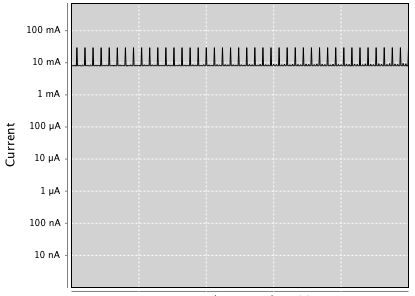
\includegraphics[width=0.5\textwidth]{images/welcome_opt.png}
\label{fig:opt}
\caption{Average current consumption of 12mA with game running with optimizations.}
\end{figure}

Pengutronix, the company responsible for porting uCLinux to the EFM32GG, claims that the distribution should be able to run as low 1.6mA in IDLE mode. Even with a lot of kernel configuration attempts, we were not able to achieve this number. 

\section{Kernel configurations}

Several kernel configuration was tested. Tickless kernel, opportunistic sleep and CPU power modes was enabled. However, none of the options gave any noticeable difference in the overall power consumption.  
\chapter{Conclusion}


% Bibliography - edit references.bib and use the \cite command in text
\bibliographystyle{plain}
\bibliography{references}
\end{document}
